\documentclass{article}
%DIF LATEXDIFF DIFFERENCE FILE
%DIF DEL manuscript.tex       Sun Jul 10 19:00:32 2022
%DIF ADD manuscript_new.tex   Wed Jul 13 17:50:40 2022
\usepackage[utf8]{inputenc}
\usepackage{caption}
\usepackage{subcaption}
\usepackage{multicol}
\usepackage{xcolor}

\usepackage{cite}


%\theoremstyle{thmstyletwo}%
\newtheorem{example}{Example}%
\newtheorem{remark}{Remark}%

%\theoremstyle{thmstylethree}%
\newtheorem{definition}{Definition}%

\newcommand{\sqrtsNN}{\mbox{$\sqrt{\mathrm{s}_{_{\mathrm{NN}}}}$}}
\newcommand{\sqrts}{\mbox{$\sqrt{\mathrm{s}}$}}
\newcommand{\axi}{$\overline{\Xi}^+$}
\newcommand{\xim}{$\Xi^-$}
%\newcommand{\xi}{$\Xi$}
\newcommand{\alam}{$\overline{\Lambda}$}
\newcommand{\sbar}{$\overline{\s}$}
\newcommand{\lam}{$\Lambda$}
\newcommand{\ks}{$\mathrm{K}^{0}_{\mathrm S}$}
\newcommand{\omm}{$\Omega^-$}
\newcommand{\aom}{$\overline{\Omega}^+$}
\newcommand{\mpt}{$\langle p_T \rangle$ }
\newcommand{\ppt}{$p_{\rm T}$}
\newcommand{\muB}{$\mu_{\rm B}$}
\newcommand{\rcp}{$R_{\textrm{\tiny{CP}}}$}

%%%%%%%%%%%%%%%%%%%%%%%%%%%%
\renewcommand{\baselinestretch}{1.12}
\renewcommand{\thefootnote}{\fnsymbol{footnote}}
\setlength{\parindent}{.5cm} \setlength{\columnsep}{.5cm}
\setlength{\oddsidemargin}{-.5cm} \setlength{\topmargin}{-1.5cm}
\setlength{\textwidth}{17.5cm} \setlength{\textheight}{23.5cm}
%%%%%%%%%%%%%%%%%%%%%%%%%%%%

\def \auau  {Au+Au}
\def \pp    {$p + p$ }
\def \llam {$\Lambda + \overline{\Lambda}$}
\def \xxi       {$\Xi^- + \overline{\Xi}^+$ }
\def \oom       {$\Omega^- + \overline{\Omega}^+$ }
\newcommand{\mean}[1]{\left\langle #1 \right\rangle}

\usepackage{graphicx}
%\usepackage{cite}

%\usepackage{lineno}
\providecommand{\keywords}[1]{\textbf{\textit{Keywords---}} #1}
\raggedbottom

\bibliographystyle{unsrt}
\usepackage{amssymb}

\usepackage{graphicx}
\usepackage{multicol}

\usepackage{lineno}
%DIF PREAMBLE EXTENSION ADDED BY LATEXDIFF
%DIF UNDERLINE PREAMBLE %DIF PREAMBLE
\RequirePackage[normalem]{ulem} %DIF PREAMBLE
\RequirePackage{color}\definecolor{RED}{rgb}{1,0,0}\definecolor{BLUE}{rgb}{0,0,1} %DIF PREAMBLE
\providecommand{\DIFadd}[1]{{\protect\color{blue}\uwave{#1}}} %DIF PREAMBLE
\providecommand{\DIFdel}[1]{{\protect\color{red}\sout{#1}}}                      %DIF PREAMBLE
%DIF SAFE PREAMBLE %DIF PREAMBLE
\providecommand{\DIFaddbegin}{} %DIF PREAMBLE
\providecommand{\DIFaddend}{} %DIF PREAMBLE
\providecommand{\DIFdelbegin}{} %DIF PREAMBLE
\providecommand{\DIFdelend}{} %DIF PREAMBLE
%DIF FLOATSAFE PREAMBLE %DIF PREAMBLE
\providecommand{\DIFaddFL}[1]{\DIFadd{#1}} %DIF PREAMBLE
\providecommand{\DIFdelFL}[1]{\DIFdel{#1}} %DIF PREAMBLE
\providecommand{\DIFaddbeginFL}{} %DIF PREAMBLE
\providecommand{\DIFaddendFL}{} %DIF PREAMBLE
\providecommand{\DIFdelbeginFL}{} %DIF PREAMBLE
\providecommand{\DIFdelendFL}{} %DIF PREAMBLE
%DIF END PREAMBLE EXTENSION ADDED BY LATEXDIFF

\begin{document}

%%%%%%%%%%%%%%%%%%%%%%%

\begin{center}
{\Large \bf A Comprehensive Study of Energy Dependence of Particle Ratios in $pp$ Collisions from SPS to LHC Energies }

\vskip1.0cm

A.~M.~Khan$^{1}$,
\DIFdelbegin \DIFdel{Junaid~Tariq$^{2}$,
Anwarzada$^{3}$, 
Ijaz Ahmed$^{3}$}%DIFDELCMD < {%%%
\footnote{\DIFdel{E-mail: ijaz.ahmed@riphah.edu.pk}}%DIFAUXCMD
\addtocounter{footnote}{-1}%DIFAUXCMD
%DIFDELCMD < }%%%
\DIFdel{,
}\DIFdelend M.~U.~Ashraf\DIFdelbegin \DIFdel{$^{4}$}\DIFdelend \DIFaddbegin \DIFadd{$^{2}$}\DIFaddend {\footnote{Email: usman.ashraf@cern.ch}}
\DIFdelbegin %DIFDELCMD < \\
%DIFDELCMD < %%%
\DIFdelend \DIFaddbegin \DIFadd{Junaid~Tariq$^{3}$,
Anwarzada$^{4}$, 
Ijaz Ahmed$^{4}$%DIF > {\footnote{E-mail: ijaz.ahmed@riphah.edu.pk}}\\
}\DIFaddend 

{\small\it 
$^1$Key Laboratory of Quark \& Lepton Physics (MOE) and Institute of Particle Physics,
Central China Normal University, Wuhan 430079, China\\
$^2$ \DIFdelbegin \DIFdel{Department of Physics, Quaid-i-Azam University, Islamabad 44000}\DIFdelend \DIFaddbegin \DIFadd{Pakistan Institute of Nuclear Science and Technology (PINSTECH), Islamabad 45650}\DIFaddend , Pakistan\\
%DIF < $^3$ Department of Physics, Riphah International University, Islamabad 44000, Pakistan\\
$^3$ Department of Physics, \DIFdelbegin \DIFdel{Riphah International }\DIFdelend \DIFaddbegin \DIFadd{Quaid-i-Azam }\DIFaddend University, Islamabad 44000, Pakistan\\
$^4$ \DIFdelbegin \DIFdel{Pakistan Institute of Nuclear Science and Technology (PINSTECH), }\DIFdelend \DIFaddbegin \DIFadd{Department of Physics, Riphah International University, }\DIFaddend Islamabad 44000, Pakistan\\


}
\end{center}


\vskip1.0cm
%%%%%%%%%%%%%%%%%%%%%%
%\linenumbers
%\date{October 2021}

%\begin{document}

%\maketitle
\begin{abstract}

A comprehensive study has been \DIFdelbegin \DIFdel{preformed }\DIFdelend \DIFaddbegin \DIFadd{performed }\DIFaddend to estimate the kaon to pion (\DIFdelbegin \DIFdel{$K^+$}\DIFdelend \DIFaddbegin \DIFadd{$K^\pm$}\DIFaddend /\DIFdelbegin \DIFdel{$\pi^+$, $K^-$/$\pi^-$) }\DIFdelend \DIFaddbegin \DIFadd{$\pi^\pm$) yield }\DIFaddend ratio and total kaon to total pion ($K$/$\pi$) \DIFaddbegin \DIFadd{yield }\DIFaddend ratio as a function of \DIFaddbegin \DIFadd{centre of mass }\DIFaddend energy in $pp$ collisions at different energies i.e., \sqrts~= 6.3, 17.3, 62.4, 200, 900 GeV, 2.76 TeV, 7 TeV, 13 TeV and 14 TeV using EPOS1.99, \DIFdelbegin \DIFdel{EPOS LHC}\DIFdelend \DIFaddbegin \DIFadd{EPOS-LHC}\DIFaddend , HIJING, \DIFdelbegin \DIFdel{QGSJET II and Sibyll }\DIFdelend \DIFaddbegin \DIFadd{QGSJETII-03 and Sibyll2.3d }\DIFaddend model simulations. \DIFaddbegin \DIFadd{NA61/SHINE experiment reported that $K^+/\pi^+$ yield ratio exhibits rapid changes at the SPS energy range. A horn like structure appears in $K/\pi$ yield ratio as a function of collision energy. }\DIFaddend Significant presence of horn in $K^+$/$\pi^+$ and $K^-$/$\pi^-$ \DIFaddbegin \DIFadd{yield }\DIFaddend ratio is suggested by experimental data at lower energies, which is confirmed by HIJING and \DIFdelbegin \DIFdel{EPOS LHC model}\DIFdelend \DIFaddbegin \DIFadd{EPOS-LHC models}\DIFaddend . A smooth increase in $K/\pi$ \DIFaddbegin \DIFadd{yield }\DIFaddend ratio is also seen at higher energies. The \DIFdelbegin \DIFdel{current }\DIFdelend model simulations predict \DIFdelbegin \DIFdel{the }\DIFdelend similar increase in \DIFdelbegin \DIFdel{the }\DIFdelend \DIFaddbegin \DIFadd{yield }\DIFaddend ratio with increasing energies. \DIFdelbegin \DIFdel{Almost all the models suggest a saturation in $K/\pi$ ratio at the LHC energies. }\DIFdelend On the basis of previous available measurements, we also \DIFdelbegin \DIFdel{give }\DIFdelend \DIFaddbegin \DIFadd{study model }\DIFaddend predictions of these \DIFaddbegin \DIFadd{yield }\DIFaddend ratios at \sqrts~= 13 and 14 TeV \DIFdelbegin \DIFdel{. All the model predictions at \sqrts~= 13 and 14 TeV }\DIFdelend \DIFaddbegin \DIFadd{where no data is available. Almost all models }\DIFaddend suggest a saturation in the \DIFdelbegin \DIFdel{ratio at higher energies }\DIFdelend \DIFaddbegin \DIFadd{yield ratio within statistical fluctuations at these energies except EPOS1.99 and QGSJETII-03 which slightly over predict the yield ratio. These systematic comparisons are helpful to apply possible constraints on various hadronic event generators to significantly improve the predictions of Standard Model physics as well as for the understanding of underlying physics mechanisms in high energy collisions}\DIFaddend . 
\DIFdelbegin \DIFdel{However, QGSJTE II predictions are higher as compared to other models.      
}\DIFdelend 


\vskip0.5cm
\DIFdelbegin \DIFdel{\keywords{collisions, simulation, function, energy, prediction}
}\DIFdelend \DIFaddbegin \DIFadd{\keywords{Hadronic event generators, $pp$ collisions, Monte-Carlo Simulation, Prediction, LHC energies}
}\DIFaddend \end{abstract}


%\maketitle
%\begin{multicols}{2}

\section{Introduction}\label{sec1}

%One of the most fundamental physical observables, which have been extensively measured and hence studied in cosmic-ray physics and hadronic colliders for many decades, are the yield and transverse momentum spectra ({\ppt}) of identified particles produced in high energy hadronic interactions~\cite{1}. At partonic level, hadrons are produced from the soft and hard scattering processes at collider energies. The interaction of two partons with large amount of momentum transfer is known as the hard scatterings which results the production of high {\ppt} particles. Theoretically, the factorization theorem based perturbative Quantum Chromodynamics (pQCD) caEPOS LHClculations explain this process~\cite{2}. At the LHC, the lower $x$ regime is probed by increasing the center of mass energy (\sqrts) which results the increase in contributions from the hard scattering processes. The dominant production of high-{\ppt} particles are from the fragmentation of gluons in the kinematic regions probed by these measurements~\cite{3,4}. On the other hand, the origin of bulk of low {\ppt} ({\ppt} $< 2$ GeV/$c$) particles are from soft scattering processes having small amount of momentum transfer. The production of particles in this regime cannot be calculated from the first principle and therefore QCD inspired phenomonological models plays a significant role for these calculations. These models are then tuned for the comparison of previous measurements and hence, low {\ppt} measurements may helpful to provide further important constraints on models.             

The nucleus-nucleus ($AA$) collisions at ultra-relativistic energies has been one of the major area of interest for experimental and theoretical physicists. \DIFdelbegin \DIFdel{The }\DIFdelend $AA$ collisions could be helpful to extract \DIFdelbegin \DIFdel{the }\DIFdelend information about the spatiotemporal evolution of multi-particle production processes, one of the primary interests in view of recent progresses in Quantum Chromodynamics (QCD). In addition to $AA$ interactions, the study of proton-proton ($pp$) collisions are also important because it provides input to \DIFdelbegin \DIFdel{the theoretical models bases on the }\DIFdelend \DIFaddbegin \DIFadd{theoretical models based on }\DIFaddend strong interactions. Another important aspect is that, it acts as a baseline to understand the $AA$ collisions at relativistic and ultra-relativistic energies. \DIFaddbegin \DIFadd{This reference is also needed for the investigation of possible initial state effects in the collisions. }\DIFaddend The production of soft particle in $pp$ interactions is sensitive to the hadronization of quark, flavor distribution inside the proton and baryon number transport. 
\DIFdelbegin \DIFdel{The study of transverse momentum (}%DIFDELCMD < {\ppt}%%%
\DIFdel{) of identified charged particle in $pp$ interactions act as a bottom-line reference to those measured in $AA$ interactions. This reference is also needed for the investigation of possible initial state effects in the collisions.    
}\DIFdelend 

The multiplicity distribution of produced particles in $pp$ collisions is one of the basic observables which shows the properties of \DIFdelbegin \DIFdel{the }\DIFdelend underlying production mechanisms of \DIFdelbegin \DIFdel{the }\DIFdelend different particles. In addition to \DIFdelbegin \DIFdel{the }\DIFdelend production of $\pi^\pm$, the production of $K^\pm$ is also of great interest due to the fact that strangeness production is a sensitive probe to study the hadronic interactions as well as hadronization in $pp$ and ultra-relativistic \DIFdelbegin \DIFdel{$NN$ }\DIFdelend \DIFaddbegin \DIFadd{$AA$ }\DIFaddend collisions. The strangeness enhancement in $AA$ collisions is suggested as a possible signature of quark-gluon plasma (QGP) ~\cite{5}. It is a fact that \DIFdelbegin \DIFdel{the }\DIFdelend initial state collisions does not contain any strange quark or strange anti-quark but \DIFdelbegin \DIFdel{the }\DIFdelend production of kaons confirms that the strange quark and anti-strange quark pair is created during the collisions between nucleons and nuclei. The nuclei collisions form a high energy density fireball which expand rapidly and \DIFdelbegin \DIFdel{an intermediate partonic phase }\DIFdelend \DIFaddbegin \DIFadd{a partonic phase of quasi free quarks and gluons}\DIFaddend , the QGP is expected to produce~\cite{6}. Therefore, \DIFdelbegin \DIFdel{the }\DIFdelend investigation of these interactions may provide useful information to distinguish between hadronic and partonic matter as well as \DIFdelbegin \DIFdel{the }\DIFdelend properties of phase transition in between.

The production of $K^\pm$ \DIFdelbegin \DIFdel{in $pp$ collisions }\DIFdelend will shed light to understand the strangeness production mechanisms in elementary \DIFaddbegin \DIFadd{($pp$) }\DIFaddend collisions~\cite{5}. In high energy collisions, \DIFdelbegin \DIFdel{the }\DIFdelend $K/\pi$ ratio \DIFaddbegin \DIFadd{is }\DIFaddend suggested as a key tool to study the strongly interacting matter by means of relative strangeness yield. Another important aspect to study this ratio is to address the \DIFdelbegin \DIFdel{the }\DIFdelend possible questions regarding the phase transition but also helps to better understand the hadronization and pre-equilibrium dynamics of the system. \DIFdelbegin \DIFdel{A horn is seen in the }\DIFdelend \DIFaddbegin \DIFadd{The data from NA61/SHINE experiment reflect rapid changes in $K^+/\pi^+$ yield ratio at the SPS energy range~\mbox{%DIFAUXCMD
\cite{NA49:2002pzu, NA49:2007stj, Pulawski:2015tka}}%DIFAUXCMD
. A horn like structure appears in }\DIFaddend $K/\pi$ \DIFdelbegin \DIFdel{ratio distribution in}\DIFdelend \DIFaddbegin \DIFadd{yield ratio as a function of collision energy as reported in~\mbox{%DIFAUXCMD
\cite{NA49:2002pzu, NA49:2007stj, Pulawski:2015tka}}%DIFAUXCMD
. Similar structure is also observed in }\DIFaddend $AA$ collisions around \sqrts~\DIFdelbegin \DIFdel{=}\DIFdelend \DIFaddbegin \DIFadd{$\approx$~}\DIFaddend 8 GeV\DIFaddbegin \DIFadd{, where one expects the transition between confined and deconfined matter with the creation of mixed phases, }\DIFaddend which may indicate the onset of deconfinement in comparison with smaller colliding systems~\DIFdelbegin \DIFdel{\mbox{%DIFAUXCMD
\cite{7}}%DIFAUXCMD
, while it could be used as a reference for the investigation of the strangeness enhancement in $pp$ collisions
}\DIFdelend \DIFaddbegin \DIFadd{\mbox{%DIFAUXCMD
\cite{Gazdzicki:2010iv, 7}}%DIFAUXCMD
. The significant difference is reported in the ratio upto \sqrts~= 200 GeV while at higher energies this difference becomes insignificant. This difference may arise due to the underlying production mechanisms of $K^+$ and $K^-$ at lower and higher energies. Two possible mechanisms are involved to study the $K^\pm$ production, first is pair production which is dominated at higher energies and the other is associated production which is dominated at lower energies. 
}\DIFaddend 


This paper presents a comparison of $K^+/\pi^+$, $K^-/\pi^-$ and $K/\pi$ \DIFdelbegin \DIFdel{ratio }\DIFdelend \DIFaddbegin \DIFadd{yield ratios from experimental data }\DIFaddend at different energies, i.e., \sqrts~= 6.3, 17.3, 62.4, 200, 900 GeV, 2.76 TeV, 13 TeV and 14 TeV \DIFdelbegin \DIFdel{with various monte-carlo model based simulations }\DIFdelend in $pp$ collisions \DIFdelbegin \DIFdel{. The data from different experiments is then compared }\DIFdelend with EPOS1.99, \DIFdelbegin \DIFdel{EPOS LHC}\DIFdelend \DIFaddbegin \DIFadd{EPOS-LHC}\DIFaddend , HIJING, \DIFdelbegin \DIFdel{QGSJET II and Sibyll }\DIFdelend \DIFaddbegin \DIFadd{QGSJETII-03 and Sibyll2.3d }\DIFaddend model simulations. The paper is organized as follows; Brief introduction of the models is presented in section~\ref{sec2}. In section~\ref{sec3} results and discussion is presented followed by conclusion in section~\ref{sec4}.   


\section{Model Details}\label{sec2}
 It is not yet possible to perform calculations with first principles of Quantum Chromodynamics (QCD) for the observables related to bulk of the produced particles at colliders in high energy interactions. Phenomenological models, relying on basic principles of Quantum Field Theory (QFT) and predictions of pQCD together with phenomenological fits, are instead used for the predictions of various observables high energy interactions~\cite{dEnterria:2011twh}. The various models used for comparisons are briefly discussed in the remaining part of this section.

%\subsection{DPMJET-III}
{\bf DPMJET}\DIFaddbegin \DIFadd{~\mbox{%DIFAUXCMD
\cite{Roesler:2000he} }%DIFAUXCMD
}\DIFaddend is based on Dual Parton Model (DPM) for the description of soft and multi-particle interactions in \DIFdelbegin \DIFdel{the }\DIFdelend high-energy collisions. Soft processes are described by pomerons exchange under the Regge theory scheme and \DIFdelbegin \DIFdel{the }\DIFdelend hard processes by using perturbative parton scattering approach. DPMJET works on the principles of multiple scattering Gribov-Glauber formalism and can be used to simulate a wide range of $hh$, $\gamma h$, $\gamma \gamma$, $AB$ and $\gamma A$ collisions for \DIFdelbegin \DIFdel{the }\DIFdelend energies ranging from few GeV to cosmic-ray interactions of the highest energy scale. The physics models and flexibility of DPMJET allows for the calculations of total, (quasi) elastic as well as production cross-sections for various colliding systems at high energies~\cite{Roesler:2000he}. The hadronic interaction model for $pp$ collisions in the DPMJET is derived from PHOJET while the fragmentation configurations are acceded from PYTHIA Lund model~\cite{ATLAS:2020bhl}. DPMJETIII \DIFaddbegin \DIFadd{used for this study }\DIFaddend integrated the features of PHOJET, DPMJETII and DTUNUC2 models with Glauber-Gribov calculations for intra-nuclear cascades, excited nuclei and various nuclear cross-sections~\cite{Roesler:2000he}. An account of DPMJET model characteristics and upgraded features is made in Refs.~\cite{Roesler:2000he, Bopp:2005cr}. 

%\subsection{EPOS1.99}
{\bf EPOS}\DIFaddbegin \DIFadd{~\mbox{%DIFAUXCMD
\cite{Pierog:2009zt} }%DIFAUXCMD
}\DIFaddend is based on a scattering approach in which partons and strings are treated consistently in a quantum mechanical framework. A high-energy hadronic interaction, in simple parton based models is considered as a “parton ladder” exchange between participants of the interaction. The “parton ladder” in EPOS has two parts, a hard-scattering part and an entirely phenomenological soft part parameterized in Regge pole fashion. Therefore, it is based on perturbative QCD, Gribov-Regge multiple scattering, and string fragmentation. \DIFdelbegin \DIFdel{EPOS LHC model has the }\DIFdelend \DIFaddbegin \DIFadd{EPOS-LHC model has }\DIFaddend same theoretical foundation as the \DIFdelbegin \DIFdel{EPOS 1.99. In addition, EPOS LHC }\DIFdelend \DIFaddbegin \DIFadd{EPOS1.99. EPOS-LHC }\DIFaddend makes a few adjustments to the parameters related to flow of the high-density core of thermalized matter created following \DIFdelbegin \DIFdel{pp }\DIFdelend \DIFaddbegin \DIFadd{$pp$ }\DIFaddend or $AA$ collisions\DIFdelbegin \DIFdel{. %DIF < In addition, EPOS includes off-shell remnants in the picture and thus can solve multi-strange baryon problem arising in the conventional interaction models. Effects related to consistent cross-section calculation with energy conservation, Cronin transverse momentum broadening, parton saturation, screening and collective behaviour in heavy-ion interactions have also been included in EPOS. The version EPOS1.99 used in this study included the non-linear effects, reduced cross section and inelasticity as compared to its previous version EPOS1.61.%
}\DIFdelend \DIFaddbegin \DIFadd{~\mbox{%DIFAUXCMD
\cite{Pierog:2013ria}}%DIFAUXCMD
. This model is implemented for the hadronization phase as modifications to the string fragmentation depending on string density in final state. Particularly, it is important to note that this model gets the relation between mean transverse momentum and charged particle multiplicity without implementation of color reconnection in comparison with models like Pythia~\mbox{%DIFAUXCMD
\cite{Sjostrand:2007gs} }%DIFAUXCMD
and Herwig~\mbox{%DIFAUXCMD
\cite{Bellm:2015jjp}}%DIFAUXCMD
. In addition, EPOS includes off-shell remnants in the picture and thus can solve multi-strange baryon problem arising in the conventional interaction models. Effects related to consistent cross-section calculation with energy conservation, Cronin transverse momentum broadening, parton saturation, screening and collective behaviour in heavy-ion interactions have also been included in EPOS. The version EPOS1.99 included the non-linear effects, reduced cross section and inelasticity as compared to its older versions. Updated versions of EPOS-LHC and EPOS1.99 are used forcurrent study. }\DIFaddend More details on EPOS model and developments included in EPOS1.99 can be found in Ref.~\cite{Pierog:2009zt}.


%\subsection{QGSJETII-04}
{ \bf QGSJET}\DIFaddbegin \DIFadd{~\mbox{%DIFAUXCMD
\cite{Ostapchenko:2007qb} }%DIFAUXCMD
}\DIFaddend hadronic interaction model is developed in the framework of Quark-Gluon String model~\cite{Engel:2011zzb}. The description of semi-hard processes as “semi-hard pomeron” approach and a scheme for incorporating the heavy-ion interactions were later included in the model~\cite{Kalmykov:1993qe}. In \DIFdelbegin \DIFdel{the }\DIFdelend QGSJET, a scattering is considered as a pomeron exchange process having two different (soft and semi-hard) components. Nucleus-Nucleus or hadron-hadron interactions are then modelled under the Gribove’s Reggeon \DIFdelbegin \DIFdel{Theory }\DIFdelend \DIFaddbegin \DIFadd{theory }\DIFaddend as multiple scattering\DIFdelbegin \DIFdel{processes and the }\DIFdelend \DIFaddbegin \DIFadd{, but there is no fluid component and }\DIFaddend Lund algorithm is used to disintegrate supercritical pomerons into strings. Abramovski Gribov Kancheli (AGK) cutting rules and optical theorem are employed to estimate the cross sections of \DIFdelbegin \DIFdel{the }\DIFdelend final states. Parton cascade overlapping at higher energies or in central collisions create significant nonlinear effects in the interactions, these effects are described as pomeron-pomeron interactions in the Raggeon Field Theory (RFT). The \DIFdelbegin \DIFdel{QGSJETII model }\DIFdelend \DIFaddbegin \DIFadd{version QGSJETII-03 used for this study }\DIFaddend has been designed to include the nonlinear effects at the fundamental level by enhanced pomeron diagrams approach~\cite{Ostapchenko:2004ss}. Further details about the QGSJET model and QGSJETII can be seen in Refs.~\DIFdelbegin \DIFdel{\mbox{%DIFAUXCMD
\cite{Ostapchenko:2004ss, Engel:2011zzb, Kalmykov:1993qe}
}%DIFAUXCMD
}\DIFdelend \DIFaddbegin \DIFadd{\mbox{%DIFAUXCMD
\cite{Ostapchenko:2007qb, Ostapchenko:2004ss, Engel:2011zzb, Kalmykov:1993qe}}%DIFAUXCMD
.
}\DIFaddend 


{\bf HIJING}\DIFaddbegin \DIFadd{~\mbox{%DIFAUXCMD
\cite{Wang:1991hta} }%DIFAUXCMD
}\DIFaddend model -- an acronym for heavy-ion jet interaction generator. The pQCD inspired model, Dual Parton model (DPM)~\cite{Capella:1979fm} for the study of jet fragmentation, while to study the effects of soft interactions at low and medium energies it uses \DIFdelbegin \DIFdel{the }\DIFdelend Lund fragmentation~\cite{Andersson:2001yu}. The particular development of this model is related to study the parton distribution functions (PDF), associated production of particles, jets and mini-jets produced in dense medium and soft excitation processes~\cite{Wang:1991hta}. HIJING can simulate multi-particles production in different systems i.e., $pp$ and $AA$ up to energy range of \DIFdelbegin \DIFdel{$\sqrt{s_{NN}}= 5-2000 $}\DIFdelend \DIFaddbegin \DIFadd{$\sqrt{s}= 5-2000 $}\DIFaddend ~GeV~\cite{Capella:1979fm, Wang:1991hta}. At the time of development, HIJING was the only model incorporates the pQCD methodology of multiple-jet processes from Pythia and other related processes including parton shadowing and jet quenching.  


%\subsection{Sibyll2.3d}
{ \bf Sibyll}\DIFaddbegin \DIFadd{~\mbox{%DIFAUXCMD
\cite{Riehn:2019jet} }%DIFAUXCMD
}\DIFaddend event generator describes the small angle production and projectile direction flow very well as it was designed majorly to understand the air showers and cosmic ray interactions in the Earth’s atmosphere. The interaction aspects related to jet production at higher {\ppt} and electroweak processes are not very well embedded in the workings of the model~\cite{Riehn:2019jet}. However, implementation of basic principles from unitarity and scattering theory empowers Sibyll to be used for phase space and energies of the interactions that are beyond the scope of modern colliders~\cite{Riehn:2017mfm}. Nonetheless, Sibyll has been used to well reproduce the LHC Run-I data~\cite{Riehn:2019jet}. The upgraded version Sibyll2.3 included better fits describing the \DIFdelbegin \DIFdel{$p/\pi/k$ }\DIFdelend \DIFaddbegin \DIFadd{$p/\pi/K$ }\DIFaddend elastic and total cross sections with inputs from experimental data. Improvement in the modeling of fragmentation region is incorporated in Sibyll2.3c. The improved version, Sibyll2.3d \DIFaddbegin \DIFadd{used for this study }\DIFaddend gives better $\pi^{+}/\pi^{0}$ ratios description along with other features that are important for the hadronization mechanism and production of muons in extensive air-showers. Refs.~\cite{Riehn:2019jet, Riehn:2017mfm, CMS:2015zrm} provide further details of the Sibyll model and its upgraded versions. 

\section{Analysis, Results and Discussion}\label{sec3}

For the current study, 0.1 million events have been generated using \DIFdelbegin \DIFdel{DPMJET III, }\DIFdelend HIJING, EPOS1.99, \DIFdelbegin \DIFdel{EPOS LHC }\DIFdelend \DIFaddbegin \DIFadd{EPOS-LHC, QGSJETII-03 }\DIFaddend and Sibyll2.3d \DIFaddbegin \DIFadd{at }\DIFaddend various beam energies i.e., \sqrts~= 6.3, 17.3, 62.4, 200, 900 GeV and 2.76 TeV, 7 TeV, 13 TeV and 14 TeV in $pp$ collisions to study the energy dependence of $K^+/\pi^+$, $K^-/\pi^-$ and $K/\pi$ \DIFdelbegin \DIFdel{ratio. Additionally, on the }\DIFdelend \DIFaddbegin \DIFadd{yield ratios. We have compared our results with the published data available so far i.e., from \sqrts~= 6.3 GeV upto 7 TeV. None of the experiment at LHC reported these ratios at energy \sqrts~ $>$ 7 TeV. LHC has started high luminosity Run-III data taking at \sqrts~= 13.6 TeV this year after more than three years of maintenance. Therefore, it is important to study the model predictions of these ratios at higher LHC energies to apply possible constraints on various hadronic event generators to improve the standard model physics predictions as well as underlying physics mechanisms in high energy collisions. On the }\DIFaddend basis of previous \DIFdelbegin \DIFdel{available energies, the prediction of these ratios are also presented }\DIFdelend \DIFaddbegin \DIFadd{published results at various energies, we also study the predictions of various models of these yield ratios }\DIFaddend at \sqrts~= 13 and 14 TeV \DIFaddbegin \DIFadd{where no data is available so far}\DIFaddend . 



\subsection{$K^+/\pi^+$ Ratio}

%DIF < The $K^+/\pi^+$ ratios has been extracted using the various above said models. 
%DIF < Table 1 shows the values of $K^+/\pi^+$ ratios obtained  from $pp$ collisions at different energies by using various MC models as mentioned earlier. These simulated results are also compared with available experimental data points at the same varied energies.  %\sqrts~= 6.3, 17.3, 62.4, 200, and 900 GeV along with the values at \sqrts~= 2.76 TeV, 7 TeV, 13 TeV and 14 TeV. 
%DIF < It can be seen from Table 1 that 
%DIF < In comparison with other MC models, the values of DPMJET III is lower as compared to other discussed models and does not show strong energy dependence at all energies. Sibyll2.3d and HIJING values are close to the experimental values from \sqrts~ $>$ 900 GeV, while slightly over predict at energy \sqrts~ $<$ 900 GeV. It has also been observed that Sibyll does not produce the simulations at \sqrts~ $<$ 10 GeV. EPOS1.99 and EPOS LHC is slightly overpredicting the experimental results upto \sqrts~ $<$ 900 GeV.   
\DIFdelbegin %DIFDELCMD < 

%DIFDELCMD < %%%
\DIFdelend The results of $K^+/\pi^+$ ratio measured by various experiments at \sqrts~= 6.3 GeV~\cite{Pulawski:2015tka}, 17.3 GeV~\cite{NA49:2009brx}, 62.4 GeV~\cite{PHENIX:2011rvu}, 200 GeV~\cite{STAR:2008med}, 900 GeV~\cite{ALICE:2011gmo} and \sqrts~ = 2.76 TeV~\cite{ALICE:2015ial}, 7 TeV~\cite{ALICE:2015ial} is \DIFdelbegin \DIFdel{compared }\DIFdelend \DIFaddbegin \DIFadd{listed }\DIFaddend in table 1. The experimental results of $K^+/\pi^+$ ratios from inelastic $pp$ collisions \sqrts~= 6.3 GeV at mid rapidity from NA61/SHINE Collaboration is presented in Ref.~\cite{Pulawski:2015tka}. It has been reported that, a rapid changes in the energy dependence of $K^+/\pi^+$ ratios is observed in the SPS energy regime~\cite{Pulawski:2015tka}. \DIFdelbegin \DIFdel{It has also been pointed out that Pythia~8, UrQMD and HSD models failed to reproduce the experimental results of NA61/SHINE satisfactorily.           
}\DIFdelend %DIF > It has also been pointed out that Pythia~8, UrQMD and HSD models failed to reproduce the experimental results of NA61/SHINE satisfactorily.           


Figure~\ref{fig1} shows \DIFdelbegin \DIFdel{the }\DIFdelend $K^+/\pi^+$ \DIFaddbegin \DIFadd{yield }\DIFaddend ratio as a function of centre of mass energy (\sqrts) in $pp$ collisions from \DIFdelbegin \DIFdel{DPMJET III, }\DIFdelend EPOS1.99, \DIFdelbegin \DIFdel{EPOS LHC}\DIFdelend \DIFaddbegin \DIFadd{EPOS-LHC}\DIFaddend , HIJING and Sibyll2.3d \DIFdelbegin \DIFdel{simulated }\DIFdelend results in comparison with \DIFdelbegin \DIFdel{the }\DIFdelend \DIFaddbegin \DIFadd{published }\DIFaddend experimental measurements. It has been observed that $K^+/\pi^+$ ratios in case of \DIFdelbegin \DIFdel{DPMJET III }\DIFdelend \DIFaddbegin \DIFadd{DPMJETIII }\DIFaddend simulations show increasing trend upto \sqrts~= 62.4 GeV and sudden decrease at \sqrts~= 200 GeV \DIFdelbegin \DIFdel{and }\DIFdelend \DIFaddbegin \DIFadd{then }\DIFaddend start to increase again with increasing energy. There is no prominent saturation is seen in case of \DIFdelbegin \DIFdel{DPMJET III }\DIFdelend \DIFaddbegin \DIFadd{DPMJETIII }\DIFaddend towards LHC energy regime. The \DIFdelbegin \DIFdel{DPMJET III }\DIFdelend \DIFaddbegin \DIFadd{DPMJETIII }\DIFaddend simulations confirm the presence of horn, which is seen in the experimental measurements. The \DIFdelbegin \DIFdel{DPMJET III }\DIFdelend \DIFaddbegin \DIFadd{DPMJETIII }\DIFaddend simulations data points for $K^+/\pi^+$ ratio is taken from Ref.~\cite{Bhattacharyya:2017rmc}. $K^+/\pi^+$ ratio extracted from the EPOS1.99 model increases with the increase in energy and start to saturate at \sqrts~ $\ge$ 13 TeV\DIFdelbegin \DIFdel{and close to the experimental measurements}\DIFdelend . While different scenario has been observed in case of \DIFdelbegin \DIFdel{EPOS LHC mode}\DIFdelend \DIFaddbegin \DIFadd{EPOS-LHC}\DIFaddend . The $K^+/\pi^+$ ratio from \DIFdelbegin \DIFdel{EPOS LHC }\DIFdelend \DIFaddbegin \DIFadd{EPOS-LHC }\DIFaddend increases upto \sqrts~= 62.4 GeV and shows a sudden decrease at \sqrts~= 200 GeV which start to increase again at higher energies indicating the horn. \DIFdelbegin \DIFdel{EPOS LHC }\DIFdelend \DIFaddbegin \DIFadd{EPOS-LHC }\DIFaddend clearly over predict the experimental data at \sqrts~= 62.4 GeV. In case of HIJING, the ratio increases upto \sqrts~= 62.4 GeV, decrease at \sqrts~= 200 GeV and increases again at higher energies reflects the presence of horn. \DIFdelbegin \DIFdel{QGSJET II and Sibyll }\DIFdelend \DIFaddbegin \DIFadd{QGSJETII-03 and Sibyll2.3d }\DIFaddend on the other hand, shows smooth increasing trend of ratios with increasing energy. It has also been observed that \DIFdelbegin \DIFdel{Sibyll }\DIFdelend \DIFaddbegin \DIFadd{Sibyll2.3d }\DIFaddend does not produce the simulations at \sqrts~ $<$ 10 GeV\DIFaddbegin \DIFadd{, therefore there is no comparison of experimental data with Sibyll2.3d at \sqrts~= 6.3 GeV}\DIFaddend . However, the abrupt increase in the ratio is seen in case of \DIFdelbegin \DIFdel{QGSJET II }\DIFdelend \DIFaddbegin \DIFadd{QGSJETII-03 }\DIFaddend in between \sqrts~= 62.4 GeV and \sqrts~= 200 GeV and the ratio saturate at higher energies. EPOS1.99, HIJING and \DIFdelbegin \DIFdel{Sibyll model }\DIFdelend \DIFaddbegin \DIFadd{Sibyll2.3d }\DIFaddend results reasonably reproduce the experimental measurements within \DIFdelbegin \DIFdel{errors}\DIFdelend \DIFaddbegin \DIFadd{statistical fluctuations}\DIFaddend . The sudden decrease in $K^+/\pi^+$ ratio is not confirmed by EPOS1.99 and \DIFdelbegin \DIFdel{Sibyll}\DIFdelend \DIFaddbegin \DIFadd{Sibyll2.3d}\DIFaddend . However, large error bars in EPOS1.99 at \sqrts~ $\le$ 62.4 GeV make it difficult to claim the presence of horn in the ratio. The experimental measurements also shows \DIFdelbegin \DIFdel{the }\DIFdelend significant presence of horn in the \DIFdelbegin \DIFdel{ratio. We also give predictions of the ratio }\DIFdelend \DIFaddbegin \DIFadd{yield ratio. The predictions of these yield ratios }\DIFaddend with various models at \sqrts~ = \DIFaddbegin \DIFadd{13 and }\DIFaddend 14 TeV \DIFaddbegin \DIFadd{where no experimental data is available so far are also presented and shown in the sub-figure~\ref{fig1} for better visualization}\DIFaddend . There is no prediction \DIFdelbegin \DIFdel{observed by DPMJET III for this ratio }\DIFdelend \DIFaddbegin \DIFadd{reported in Ref.~\mbox{%DIFAUXCMD
\cite{Bhattacharyya:2017rmc} }%DIFAUXCMD
from DPMJETIII model of these ratios }\DIFaddend at \sqrts~ =\DIFaddbegin \DIFadd{~13 and }\DIFaddend 14 TeV\DIFdelbegin \DIFdel{, while QGSJET II values of ratio is significantly }\DIFdelend \DIFaddbegin \DIFadd{. The predictions of EPOS1.99 and QGSJETII-03 are }\DIFaddend higher as compared to the other models\DIFdelbegin \DIFdel{under study. }\DIFdelend \DIFaddbegin \DIFadd{. However, EPOS-LHC, Sibyll2.3d and HIJING model predictions show saturation in the yield ratios at \sqrts~ = 13 and 14 TeV. 
}\DIFaddend 


\begin{figure}[ht!]
\begin{center}
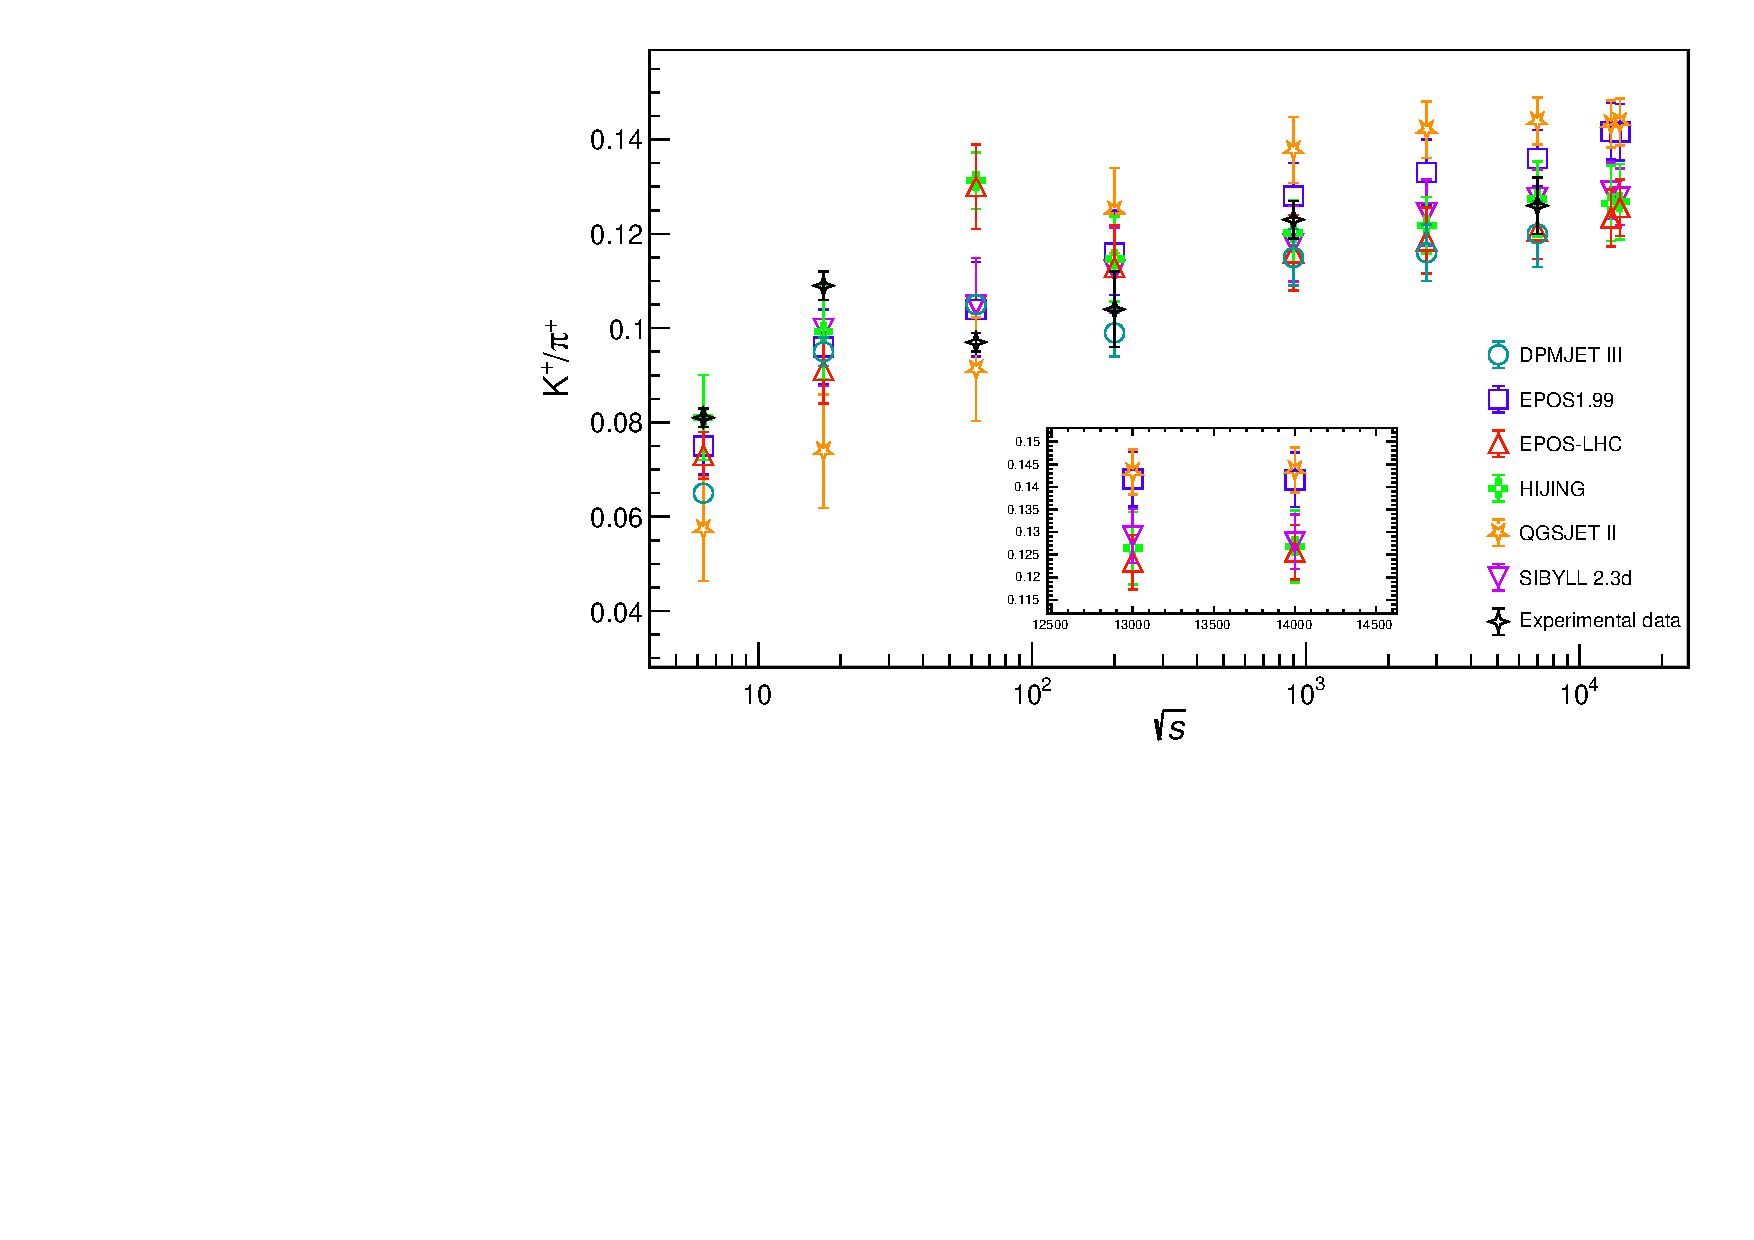
\includegraphics[width=0.8\textwidth]{new_k+_pi+.pdf}
\caption{ \DIFaddbeginFL \DIFaddFL{Energy dependence of }\DIFaddendFL $K^+/\pi^+$ \DIFaddbeginFL \DIFaddFL{yield }\DIFaddendFL ratio \DIFdelbeginFL \DIFdelFL{vs function of energy }\DIFdelendFL at \sqrts~= 6.3 GeV upto \sqrts~= 14 TeV \DIFaddbeginFL \DIFaddFL{in $pp$ collisions }\DIFaddendFL from \DIFdelbeginFL \DIFdelFL{DPMJET III}\DIFdelendFL \DIFaddbeginFL \DIFaddFL{DPMJETIII}\DIFaddendFL , EPOS1.99, \DIFdelbeginFL \DIFdelFL{EPOS LHC}\DIFdelendFL \DIFaddbeginFL \DIFaddFL{EPOS-LHC}\DIFaddendFL , HIJING\DIFaddbeginFL \DIFaddFL{, QGSJETII-03 }\DIFaddendFL and \DIFdelbeginFL \DIFdelFL{Sibyll in comparison }\DIFdelendFL \DIFaddbeginFL \DIFaddFL{Sibyll2.3d compared }\DIFaddendFL with the experimental \DIFdelbeginFL \DIFdelFL{results }\DIFdelendFL \DIFaddbeginFL \DIFaddFL{data (where available). The model predictions at \sqrts~ = 13 and 14 TeV are shown }\DIFaddendFL in \DIFdelbeginFL \DIFdelFL{$pp$ collisions}\DIFdelendFL \DIFaddbeginFL \DIFaddFL{sub-pad for better visualization}\DIFaddendFL .}
\label{fig1}
\end{center}
\end{figure}

\input table1.tex

\subsection{$K^-/\pi^-$ Ratio}\label{subsec1}

The energy dependence of $K^-/\pi^-$ ratio is computed using \DIFdelbegin \DIFdel{simulated data from various  above discussed model based event generators }\DIFdelend \DIFaddbegin \DIFadd{HIJING, SIbyll2.3d, EPOS-LHC, DPMEJETIII and QGSJETII-03 model simulations }\DIFaddend at \sqrts~= 6.3 GeV -- 14 TeV in $pp$ collisions. \DIFdelbegin \DIFdel{The resulted values of the ratio from simulations are listed in table 2 and it is observed that, the $K^-/\pi^-$ ratio from DPMJET III simulations is comparatively lower with respect to other models and EPOS1.99 is over predicting the ratio at \sqrts~ $\ge$ 62.4 GeV. HIJING, SIbyll, EPOS LHC and DPMEJET III results are compareable.  
}%DIFDELCMD < 

%DIFDELCMD < %%%
\DIFdelend %DIF > The resulted values of the ratio from simulations are listed in table 2 and it is observed that, the $K^-/\pi^-$ ratio from DPMJET III simulations is comparatively lower with respect to other models and EPOS1.99 is over predicting the ratio at \sqrts~ $\ge$ 62.4 GeV. HIJING, SIbyll, EPOS LHC and DPMEJET III results are compareable.  
Figure~\ref{fig2} presents \DIFdelbegin \DIFdel{the }\DIFdelend $K^-/\pi^-$ ratio \DIFdelbegin \DIFdel{vs }\DIFdelend \DIFaddbegin \DIFadd{as a function of }\DIFaddend energy from various model simulations in comparison with the experimental data. At lower energies \sqrts~ $\le$ 200 GeV, the \DIFdelbegin \DIFdel{DPMJET III }\DIFdelend \DIFaddbegin \DIFadd{DPMJETIII }\DIFaddend value is increasing with energy and \DIFdelbegin \DIFdel{sudden drop is seen }\DIFdelend \DIFaddbegin \DIFadd{drop suddenly }\DIFaddend at \sqrts~= 900 GeV and \DIFdelbegin \DIFdel{increases }\DIFdelend \DIFaddbegin \DIFadd{starts to increase }\DIFaddend again at higher energies \DIFdelbegin \DIFdel{shows }\DIFdelend \DIFaddbegin \DIFadd{showing }\DIFaddend the presence of horn \DIFdelbegin \DIFdel{, while UrQMD fails}\DIFdelend \DIFaddbegin \DIFadd{as observed in the energy dependence of $K^+/\pi^+$ yield ratios}\DIFaddend ~\cite{Bhattacharyya:2017rmc}. In case of HIJING and \DIFdelbegin \DIFdel{EPOS LHC the value of }\DIFdelend \DIFaddbegin \DIFadd{EPOS-LHC the }\DIFaddend ratio increases with energy upto \sqrts~ $\le$ 62.4 GeV and decreases suddenly at \sqrts~= 200 GeV and \DIFdelbegin \DIFdel{increases }\DIFdelend \DIFaddbegin \DIFadd{start to increase }\DIFaddend again at higher energies which confirms the experimental claim of the presence of horn\DIFaddbegin \DIFadd{~\mbox{%DIFAUXCMD
\cite{NA49:2002pzu, NA49:2007stj, Pulawski:2015tka}}%DIFAUXCMD
}\DIFaddend . It has also been observed that at \sqrts~= 62.4 GeV, HIJING and \DIFdelbegin \DIFdel{EPOS LHC }\DIFdelend \DIFaddbegin \DIFadd{EPOS-LHC }\DIFaddend clearly over predict the experimental results while a nice comparison at rest of energies. \DIFaddbegin \DIFadd{The ratio from }\DIFaddend EPOS1.99 and \DIFdelbegin \DIFdel{Sibyll values of the ratio }\DIFdelend \DIFaddbegin \DIFadd{Sibyll2.3d models }\DIFaddend increases smoothly with the increase in energy and fails to shows the horn structure. On the other hand, \DIFdelbegin \DIFdel{QGSJET II values of the }\DIFdelend \DIFaddbegin \DIFadd{QGSJETII-03 values of }\DIFaddend ratio smoothly increase upto \sqrts~ $\le$ 62.4 GeV and shows a sudden increase which continues towards higher energies. The \DIFdelbegin \DIFdel{ratio in case of all discussed models start to saturate at higher energy regimes. Almost all the models predict similar }\DIFdelend \DIFaddbegin \DIFadd{predictions of }\DIFaddend $K^-/\pi^-$ \DIFdelbegin \DIFdel{ratio }\DIFdelend \DIFaddbegin \DIFadd{yield ratio from EPOS1.99 and QGSJETII-03 at \sqrts~ = 13 and 14 TeV are slightly higher as compared to other models. However, EPOS-LHC, Sibyll2.3d and HIJING model predictions show saturation in the yield ratios }\DIFaddend at \sqrts~ = \DIFaddbegin \DIFadd{13 and }\DIFaddend 14 TeV \DIFdelbegin \DIFdel{, while QGSJET II values are relatively higher}\DIFdelend \DIFaddbegin \DIFadd{and are in good agreement with the published data at lower energies within statistical fluctuations}\DIFaddend . 


It is important to note that the data from experiments of $K^+/\pi^+$ and $K^-/\pi^-$ ratio \DIFdelbegin \DIFdel{vs }\DIFdelend \DIFaddbegin \DIFadd{as a function of }\DIFaddend energy confirm the presence of horn which is also observed in HIJING, \DIFdelbegin \DIFdel{DPMJET III and EPOS LHC model, while the rest of models do not }\DIFdelend \DIFaddbegin \DIFadd{DPMJETIII and EPOS-LHC models, while rest of the models }\DIFaddend significantly fails to describe the \DIFaddbegin \DIFadd{horn }\DIFaddend structure. This observed difference may be due to the difference in different models used for current study. In HIJING, Pythia approach to multiple jet processes and \DIFdelbegin \DIFdel{the }\DIFdelend nuclear effects for example\DIFaddbegin \DIFadd{, }\DIFaddend jet quenching and parton shadowing is incorporated. The multiple string phenomenological approach exchanges the multiple soft gluons between the quarks or di-quarks present in hadrons which further lead to the \DIFdelbegin \DIFdel{longitudnally }\DIFdelend \DIFaddbegin \DIFadd{longitudinally }\DIFaddend oriented string-like excitations of those hadrons are also implemented in the HIJING. In order to fix the effect if color flow, valence quarks replaces the flavour of final scattered quark or di-quark. Due to the reason that gluon jets are dominated in $K/\pi$ ratio at intermediate {\ppt} and the ratio is observed to be not sensitive to this~\cite{Sjostrand:1987su, Werner:1988yt, Wang:1991hta}. \DIFdelbegin \DIFdel{DPMJET III, EPOSQGSJET and Sibyll }\DIFdelend \DIFaddbegin \DIFadd{DPMJETIII, EPOS, QGSJETII-03 and Sibyll2.3d }\DIFaddend are hadronic interaction models and are based on Gribov Reggeon approach of Pomeron exchange in multiple scatterings. The exchange of individual pomeron occur independently in \DIFdelbegin \DIFdel{QGSJET }\DIFdelend \DIFaddbegin \DIFadd{QGSJETII }\DIFaddend model which is not true at higher energies where strong overlap of parton cascade exists which further interact with each other. This could be the reason of \DIFdelbegin \DIFdel{overpredictig both the }\DIFdelend \DIFaddbegin \DIFadd{overprediction of both }\DIFaddend ratio at higher energies~\cite{Thakuria:2012ie}. \DIFdelbegin \DIFdel{SImilar }\DIFdelend \DIFaddbegin \DIFadd{Similar }\DIFaddend to HIJING, \DIFdelbegin \DIFdel{Sibyll also incorporate the }\DIFdelend \DIFaddbegin \DIFadd{Sibyll2.3d also incorporate }\DIFaddend many concepts of Dual Parton Model. Compared to other models, a pomeron amplitude is not explicitly implemented in \DIFdelbegin \DIFdel{Sibyll}\DIFdelend \DIFaddbegin \DIFadd{Sibyll2.3d}\DIFaddend . Quantum mechanical model of multiple scattering, EPOS, is based on strings and partons. The production of particles and cross-section observed to be consistent with \DIFdelbegin \DIFdel{the }\DIFdelend conservation of energy in EPOS. \DIFdelbegin \DIFdel{DPMJET III}\DIFdelend \DIFaddbegin \DIFadd{DPMJETIII}\DIFaddend , a Hadronic transport model \DIFaddbegin \DIFadd{is }\DIFaddend based on the interactions of strings. The collisions of particles are described through the color exchange and momentum in partons \DIFaddbegin \DIFadd{both }\DIFaddend in target and projectile. \DIFdelbegin \DIFdel{These exchanges }\DIFdelend \DIFaddbegin \DIFadd{This }\DIFaddend results colorless objects to be joined with these partons which we called ropes, flux tubes or strings.     


\begin{figure}[ht!]
\begin{center}
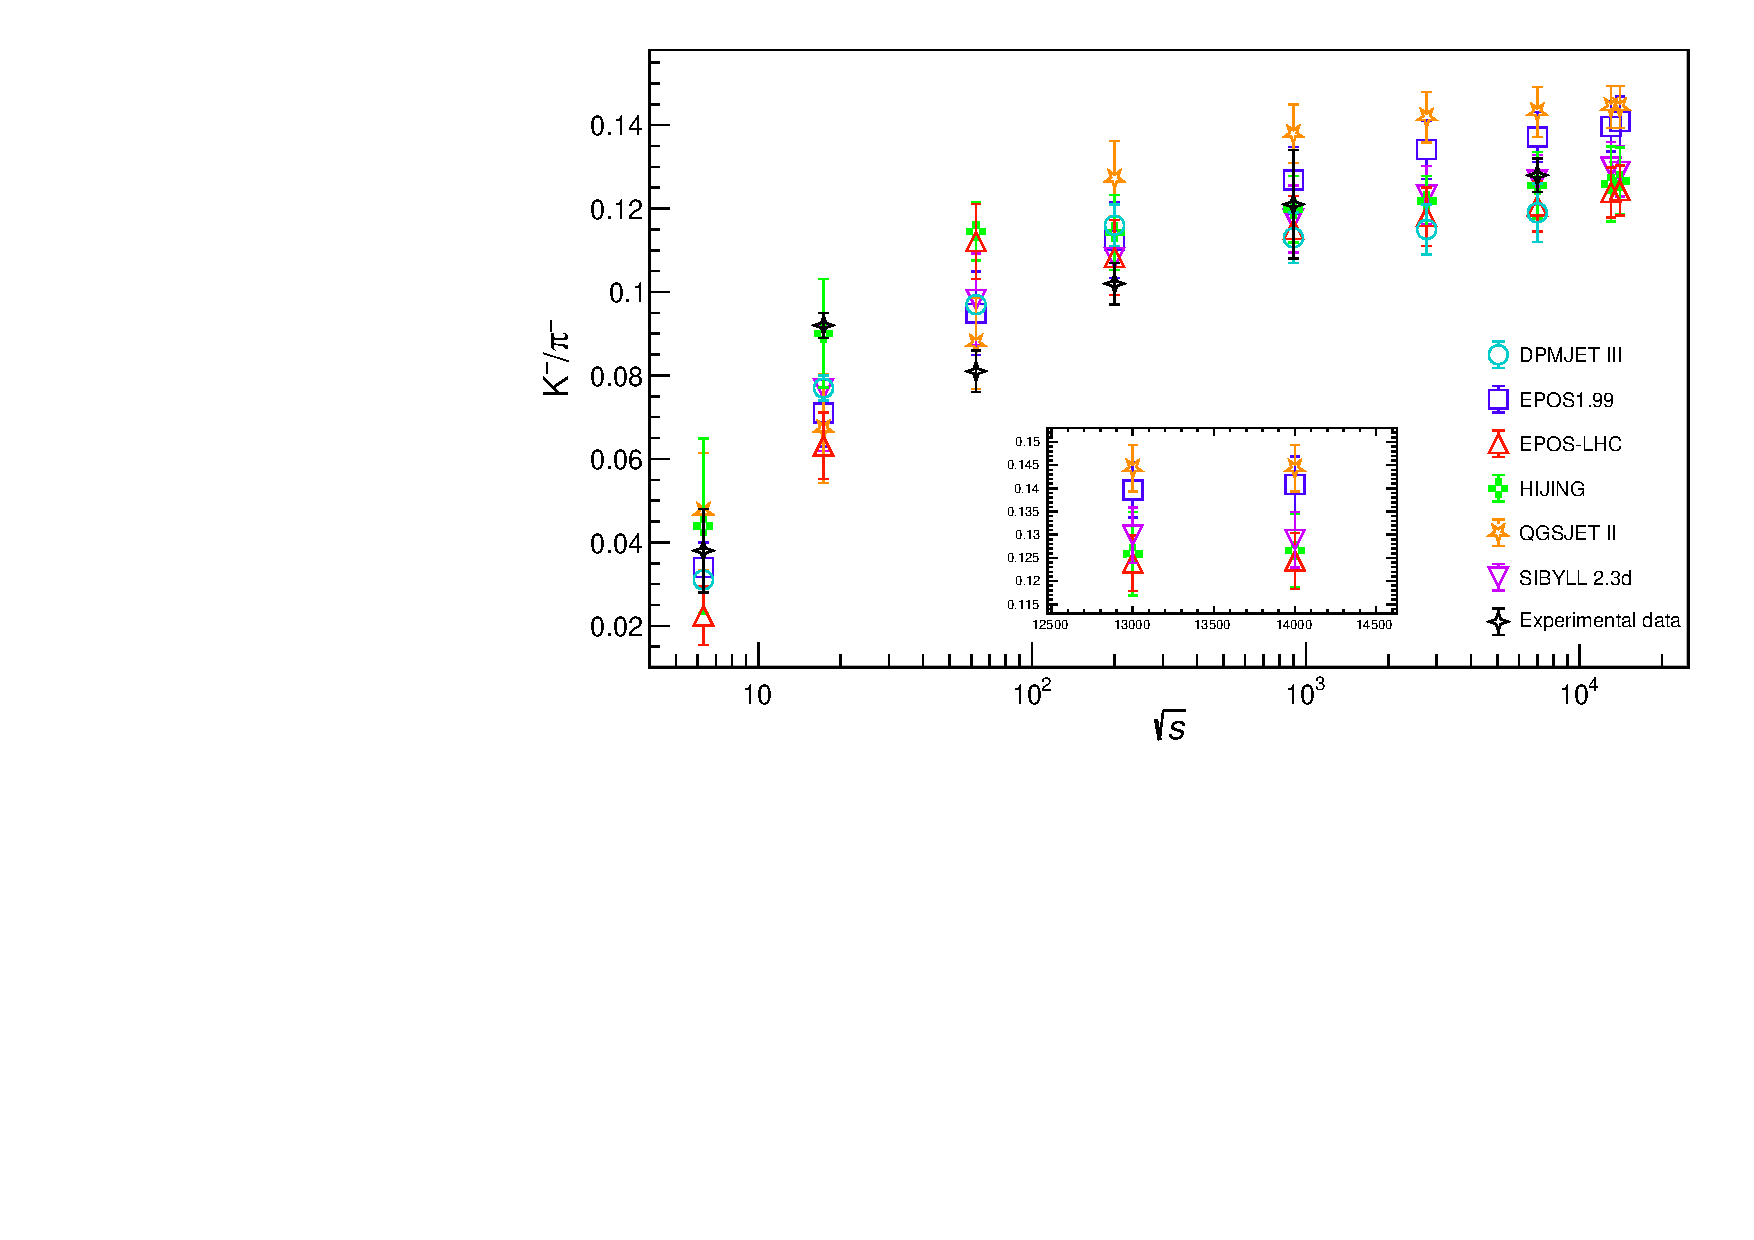
\includegraphics[width=0.8\textwidth]{new_k-_pi-.pdf}
\caption{ \DIFaddbeginFL \DIFaddFL{Energy dependence of }\DIFaddendFL $K^-/\pi^-$ \DIFaddbeginFL \DIFaddFL{yield }\DIFaddendFL ratio \DIFdelbeginFL \DIFdelFL{vs function of energy }\DIFdelendFL at \sqrts~= 6.3 GeV upto \sqrts~= 14 TeV \DIFaddbeginFL \DIFaddFL{in $pp$ collisions }\DIFaddendFL from \DIFdelbeginFL \DIFdelFL{DPMJET III}\DIFdelendFL \DIFaddbeginFL \DIFaddFL{DPMJETIII}\DIFaddendFL , EPOS1.99, \DIFdelbeginFL \DIFdelFL{EPOS LHC}\DIFdelendFL \DIFaddbeginFL \DIFaddFL{EPOS-LHC}\DIFaddendFL , HIJING\DIFaddbeginFL \DIFaddFL{, QGSJETII-03 }\DIFaddendFL and \DIFdelbeginFL \DIFdelFL{Sibyll in comparison }\DIFdelendFL \DIFaddbeginFL \DIFaddFL{Sibyll2.3d compared }\DIFaddendFL with the experimental \DIFdelbeginFL \DIFdelFL{results }\DIFdelendFL \DIFaddbeginFL \DIFaddFL{data (where available). The model predictions at \sqrts~ = 13 and 14 TeV are shown }\DIFaddendFL in \DIFdelbeginFL \DIFdelFL{$pp$ collisions}\DIFdelendFL \DIFaddbeginFL \DIFaddFL{sub-pad for better visualization}\DIFaddendFL .}

\label{fig2}
\end{center}
\end{figure}


It is important to mention that the presence of horn in $K^\pm/\pi^\pm$ ratio in experimental measurements at low energy regime is confirmed by various experiments. \DIFdelbegin \DIFdel{In }\DIFdelend \DIFaddbegin \DIFadd{The }\DIFaddend hadronic models which \DIFdelbegin \DIFdel{confirms }\DIFdelend \DIFaddbegin \DIFadd{confirm }\DIFaddend the presence of this structure at low energies, two long strings along with valence quark are present at the end and therefore, the contribution of SCET-soft sea quark in \DIFdelbegin \DIFdel{the }\DIFdelend resulted particle with low $K^\pm/\pi^\pm$ are already given in Pythia. The fits to cross-section explains the entrance of additional strings at higher energies. The partons in this case are considered like a minijet extension of pQCD events at larger {\ppt} and a continuous transition is expected at cutoff {\ppt} which could results the large {\ppt} and hence larger ratio in case of particles at sea string ends. At reaching \DIFdelbegin \DIFdel{the energy where the }\DIFdelend \DIFaddbegin \DIFadd{energy where }\DIFaddend new and shorter strings just arrived, there is sizeable fraction of those produced particles which contain \DIFdelbegin \DIFdel{the }\DIFdelend string end partons. These strings are then increases and gets longer with \DIFaddbegin \DIFadd{the }\DIFaddend increase in energy and it is expected that the influence of these strings gets weaker which results the decrease in $K^\pm/\pi^\pm$ ratio~\cite{Bhattacharyya:2017rmc}. This case is different in heavy-ion collisions due to the enhancement in the new chains as the results of collision of several nucleons with \DIFdelbegin \DIFdel{the }\DIFdelend target and conversely. The newly produced shorter strings results enhancement in \DIFdelbegin \DIFdel{the }\DIFdelend $K^\pm/\pi^\pm$ ratio. There is no significant effect from the fusion of strings and rescattering. Due to the presence of uncertainty in \DIFdelbegin \DIFdel{the }\DIFdelend parameterization relatd to sea strings, the position of this horn is not a robust prediction.  


\input table2.tex
When comparing Tables 1 and 2, there exists significant difference in \DIFdelbegin \DIFdel{the }\DIFdelend both ratios from almost all of the \DIFdelbegin \DIFdel{studied models }\DIFdelend \DIFaddbegin \DIFadd{models under study }\DIFaddend upto \sqrts~= 200 GeV and starts to saturate and hence the no significant difference is observed towards higher energies (\sqrts~= 900 GeV -- 14 TeV). Insignificant difference between the ratios has been observed in case of experimental measurements. This difference may be due to the underlying production mechanisms of $K^+$ and $K^-$. Two possible mechanisms are involved to study the $K^\pm$ production study, pair production and associated production mechanism. Kaon production is heavily influenced by associated production of $s$ and $\bar s$ quark pairs. Since, there is no kaon production through the $\Delta$ channel and hence $K^+$ are produced through $N + N \rightarrow N + X + K^+$ and $\pi + N \rightarrow X + K^+$, where, \DIFdelbegin \DIFdel{X }\DIFdelend \DIFaddbegin \DIFadd{$X$ }\DIFaddend is either {\lam} or $\Xi$ hyperon and \DIFdelbegin \DIFdel{N }\DIFdelend \DIFaddbegin \DIFadd{$N$ }\DIFaddend is the nucleon. The energy threshold for $N + N \rightarrow N + \Lambda + K$ is significantly lower than thermal production of kaon pairs. The pair production process to produce $K^+$ and $K^-$ is $N + N \rightarrow N + N + K^+ + K^-$. Kaon production in association with a $\Lambda$ is only available to $K^+$ and $K^0$ due to spin degeneracies. The associated production \DIFdelbegin \DIFdel{is dominated }\DIFdelend \DIFaddbegin \DIFadd{dominates }\DIFaddend at lower energies and pair production dominates at higher energies in which significantly same number or $K^+$ and $K^-$ are produced. Due to the higher threshold a steeper excitation function of $K^-$ is observed as compared to $K^+$ and therefore, the production cross-section of $K^-$ increases faster at higher energies to that of $K^+$ which results increase in $K^-/\pi^-$ ratio.           






\subsection{$K/\pi$ Ratio}

We have also extracted the $K/\pi$ (($K^+ + K^-$)/($\pi^+ + \pi^-$)) \DIFaddbegin \DIFadd{yield }\DIFaddend ratio in $pp$ collisions at various energies using above discussed models. These results are then compared with the $K/\pi$ ratio measured by different experiments~\cite{Pulawski:2015tka, NA49:2009brx, PHENIX:2011rvu, STAR:2008med, ALICE:2011gmo, ALICE:2015ial}. The extracted $K/\pi$ ratio from models as well as experimental values are listed in Table 3.     

Figure~\ref{fig3} presents \DIFdelbegin \DIFdel{the }\DIFdelend comparison of $K/\pi$ \DIFdelbegin \DIFdel{multiplicity }\DIFdelend \DIFaddbegin \DIFadd{yield }\DIFaddend ratio from models \DIFdelbegin \DIFdel{to that experimental results}\DIFdelend \DIFaddbegin \DIFadd{with experimental measurements}\DIFaddend . There is smooth increase in the ratio observed in experimental measurements for all energies and almost becomes independent of energy from \sqrts~= 200 GeV. Similar to experimental data, almost all the \DIFdelbegin \DIFdel{studied }\DIFdelend models starts to saturate from \sqrts~ $>$ 900 GeV. At \sqrts~ $<$ 200 GeV, EPOS1.99 and \DIFdelbegin \DIFdel{QGSJET II values are compareable }\DIFdelend \DIFaddbegin \DIFadd{QGSJETII-03 values are comparable }\DIFaddend with data while start to over predict at higher energies. \DIFdelbegin \DIFdel{Sibyll}\DIFdelend \DIFaddbegin \DIFadd{Sibyll2.3d}\DIFaddend , HIJING and \DIFdelbegin \DIFdel{EPOS LHC }\DIFdelend \DIFaddbegin \DIFadd{EPOS-LHC }\DIFaddend values of the ratio are in good agreement with experimental data at almost all of energies. While HIJING and \DIFdelbegin \DIFdel{EPOS LHC }\DIFdelend \DIFaddbegin \DIFadd{EPOS-LHC }\DIFaddend values of the ratio is almost the same and over predict the data at \sqrts~= 200 GeV. \DIFdelbegin \DIFdel{QGSJET II }\DIFdelend \DIFaddbegin \DIFadd{QGSJETII-03 }\DIFaddend values at \sqrts~ $\le$ 62.4 GeV seems to be lower as compared to experimental data and over estimate the data at higher energies. Overall, the $K/\pi$ from the models are in good agreement with experimental data \DIFaddbegin \DIFadd{within statistical fluctuations }\DIFaddend and saturation is see at higher energies. The predictions of various models at \sqrts~= 13 and 14 TeV suggest that the experimental data should be increasing and lie around the values observed from the model simulations.         


\DIFdelbegin \DIFdel{The $K/\pi$ ratio in $pp$ collisions at various RHIC and LHC energies from PACIAE model based on Pythia agrees with NA49 Experimental results~\mbox{%DIFAUXCMD
\cite{Long:2011tk}}%DIFAUXCMD
. The ratio is observed to be increasing with increasing energies. Our study with various model predictions have similar findings at lower as well as higher energies. The possible physics message has already been discussed in above section~\ref{subsec1}.  
}\DIFdelend %DIF > The $K/\pi$ ratio in $pp$ collisions at various RHIC and LHC energies from PACIAE model based on Pythia agrees with NA49 Experimental results~\cite{Long:2011tk}. The ratio is observed to be increasing with increasing energies. Our study with various model predictions have similar findings at lower as well as higher energies. The possible physics message has already been discussed in above section~\ref{subsec1}.  



\begin{figure}[ht!]
\begin{center}
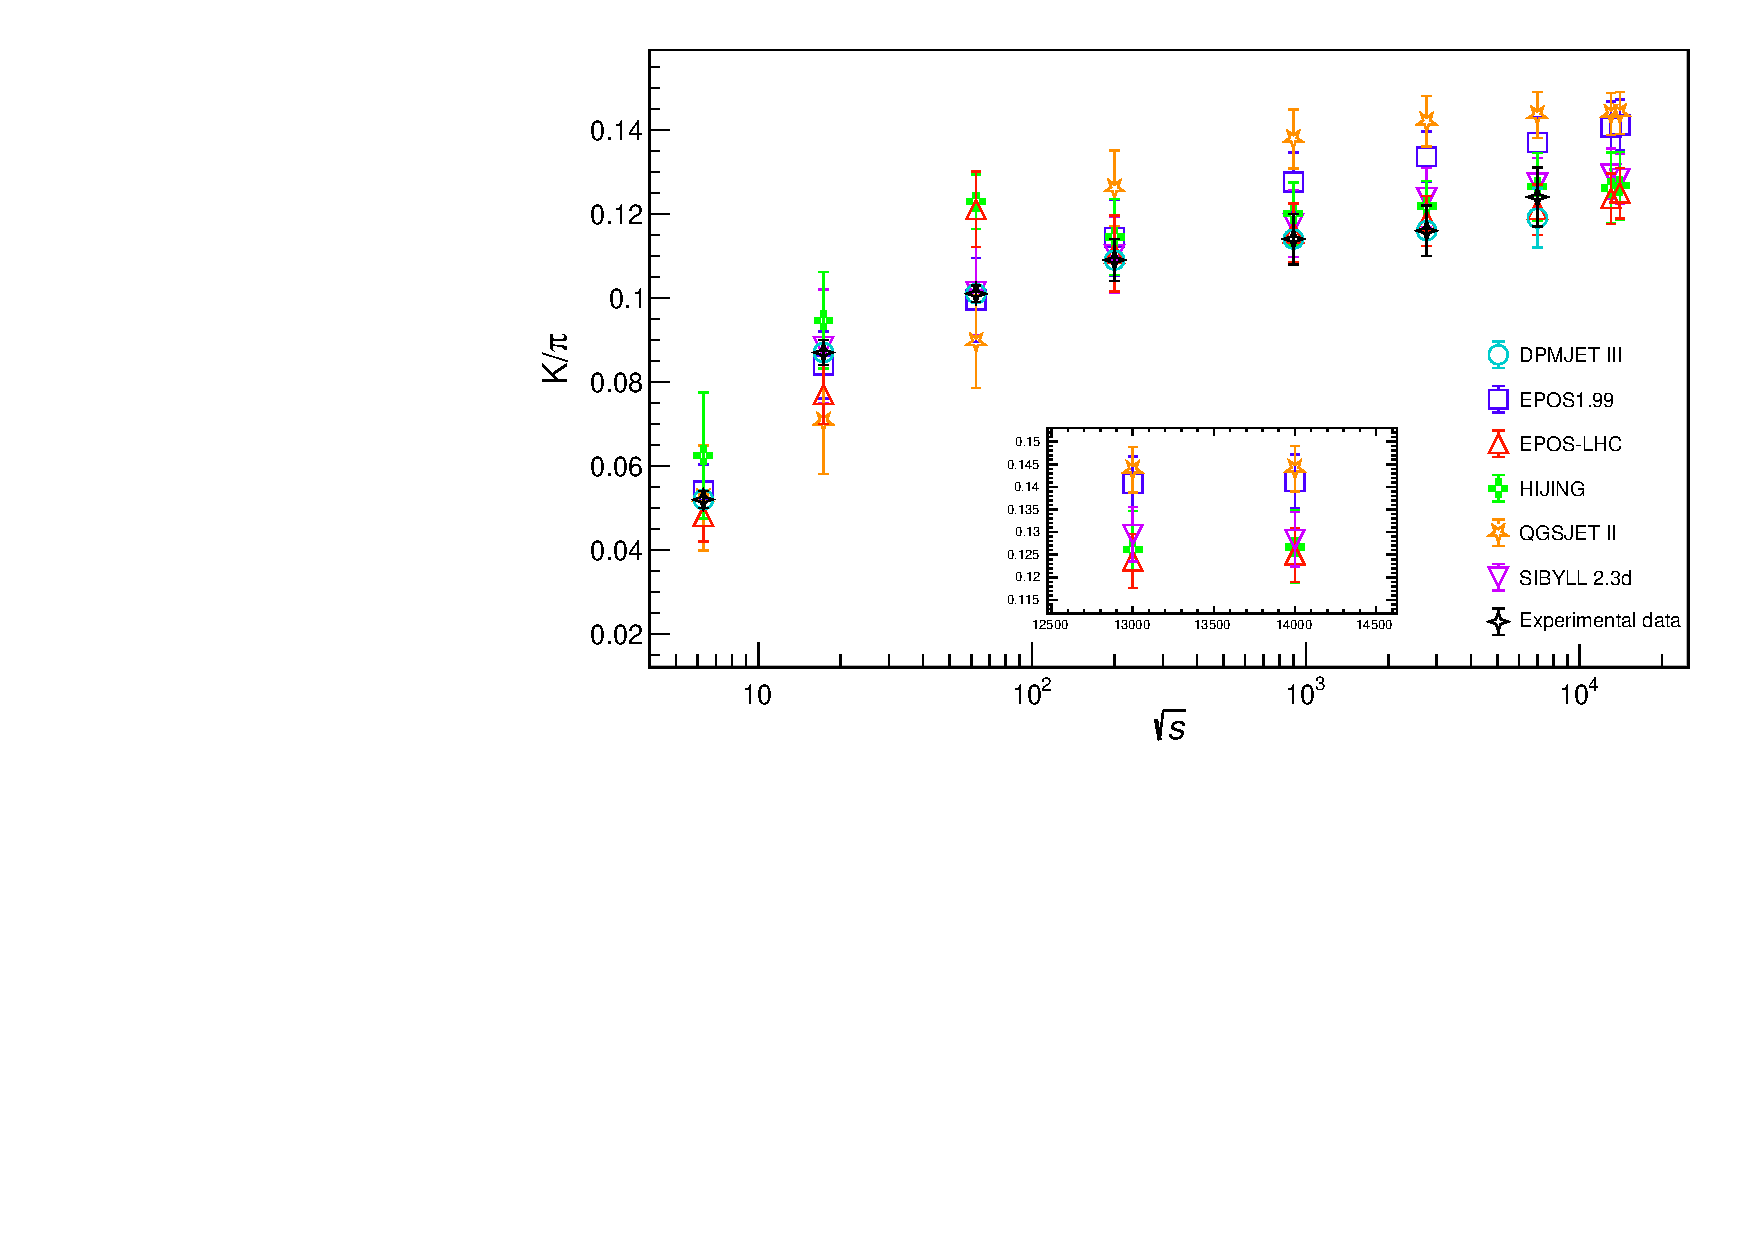
\includegraphics[width=0.8\textwidth]{new_K_pi.pdf}
\caption{ \DIFaddbeginFL \DIFaddFL{Energy dependence of }\DIFaddendFL $K/\pi$ \DIFaddbeginFL \DIFaddFL{yield }\DIFaddendFL ratio \DIFdelbeginFL \DIFdelFL{vs function of energy }\DIFdelendFL at \sqrts~= 6.3 GeV upto \sqrts~= 14 TeV \DIFaddbeginFL \DIFaddFL{in $pp$ collisions }\DIFaddendFL from \DIFdelbeginFL \DIFdelFL{DPMJET III}\DIFdelendFL \DIFaddbeginFL \DIFaddFL{DPMJETIII}\DIFaddendFL , EPOS1.99, \DIFdelbeginFL \DIFdelFL{EPOS LHC}\DIFdelendFL \DIFaddbeginFL \DIFaddFL{EPOS-LHC}\DIFaddendFL , HIJING\DIFaddbeginFL \DIFaddFL{, QGSJETII-03 }\DIFaddendFL and \DIFdelbeginFL \DIFdelFL{Sibyll in comparison }\DIFdelendFL \DIFaddbeginFL \DIFaddFL{Sibyll2.3d compared }\DIFaddendFL with the experimental \DIFdelbeginFL \DIFdelFL{results }\DIFdelendFL \DIFaddbeginFL \DIFaddFL{data (where available). The model predictions at \sqrts~ = 13 and 14 TeV are shown }\DIFaddendFL in \DIFdelbeginFL \DIFdelFL{$pp$ collisions}\DIFdelendFL \DIFaddbeginFL \DIFaddFL{sub-pad for better visualization}\DIFaddendFL .}
\label{fig3}
\end{center}
\end{figure}

\input table3.tex

\section{Conclusion}\label{sec4}


A systematic and comprehensive study has been performed \DIFdelbegin \DIFdel{in order }\DIFdelend to calculate the $K^+/\pi^+$, $K^-/\pi^-$ and $K/\pi$ (($K^+ + K^-$\DIFdelbegin \DIFdel{section}\DIFdelend )/($\pi^+ + \pi^-$)) \DIFdelbegin \DIFdel{ratio }\DIFdelend \DIFaddbegin \DIFadd{yield ratios }\DIFaddend as a function of energy in $pp$ collisions at various energies using different model simulations. A good agreement between the model predictions and experimental data has been observed\DIFdelbegin \DIFdel{in many of the studied models}\DIFdelend . The difference in both ratios ($K^+/\pi^+$, $K^-/\pi^-$) is observed in experimental measurements and model simulations from \sqrts~= 6.3 GeV to \sqrts~= 200 GeV which becomes insignificant at higher LHC energies. The experimental data suggest the presence of horn-like structure at lower energies\DIFdelbegin \DIFdel{and HIJING and EPOS LHC also suggest the }\DIFdelend \DIFaddbegin \DIFadd{. HIJING and EPOS-LHC also suggest }\DIFaddend similar findings. The production mechanism of kaon plays an important role to study this horn-like structure. There are mainly two mechanisms involved, associated production which is dominated at lower energies and pair production is dominated at higher energies. There may be a possible cross-over between these two mechanisms at energy $\approx$ \sqrts~= 54.4 GeV as reported in Ref.~\cite{Ashraf:2021nkb}\DIFdelbegin \DIFdel{in case of heavy-ion collisions}\DIFdelend . The experimental results of $K/\pi$ (($K^+ + K^-$)/($\pi^+ + \pi^-$)) \DIFaddbegin \DIFadd{yield }\DIFaddend ratio does not show the presence of horn-like structure and smoothly increasing with increasing energies. However, most of the model simulations has similar findings \DIFdelbegin \DIFdel{to }\DIFdelend \DIFaddbegin \DIFadd{as }\DIFaddend that of data except HIJING and \DIFdelbegin \DIFdel{EPOS LHC}\DIFdelend \DIFaddbegin \DIFadd{EPOS-LHC}\DIFaddend , which slightly over estimate the data at \sqrts~= 62.4 GeV. It has also been observed that the ratio \DIFdelbegin \DIFdel{at all the }\DIFdelend \DIFaddbegin \DIFadd{from all }\DIFaddend model simulations start to saturate at LHC energies. \DIFdelbegin \DIFdel{We also made }\DIFdelend \DIFaddbegin \DIFadd{The }\DIFaddend predictions of these ratios from various model simulations at \sqrts~= 13 and 14 TeV \DIFaddbegin \DIFadd{is also studied }\DIFaddend on the bases of previous available data. These predictions suggest \DIFdelbegin \DIFdel{the saturation }\DIFdelend \DIFaddbegin \DIFadd{saturation in the yield ratios }\DIFaddend at higher energies.  

\vskip0.5cm
\textbf{Acknowledgement}\\
The authors would like to show our gratitude to the Ms. Sumaira Ikram from Riphah International University, Mr. Muhammad Salman Ashraf from Institute of Space Technology, Mr. Sudheer Muhammad from Quaid-e-Azam University, Islamabad\DIFaddbegin \DIFadd{, }\DIFaddend Pakistan for sharing their pearls of wisdom with us during the course of this research. 

\vskip0.5cm
\textbf{Availability of Data and Material}\\
The authors declare that all the supported data of this study are available within the article.


%\begin{thebibliography}{}
%\bibitem{}
\input bib.tex%
%\end{thebibliography}



%\end{multicols}


%https://arxiv.org/pdf/1101.5596.pdf

\end{document}
